%!TEX TS-program = pdflatex
%!TEX encoding = UTF-8 Unicode

% Template borrowed from Jeff Erickson via Kyle Fox

\documentclass[11pt]{article}
\usepackage{jeffe,handout,graphicx}
\usepackage[utf8]{inputenc}		% Allow some non-ASCII Unicode in source
\usepackage{xcolor}
\usepackage{mdframed}
\usepackage{arydshln}
\usepackage[normalem]{ulem}
\usepackage{bigdelim}
\usepackage{listings}
\usepackage{float}
\usepackage{tabularray}
\usepackage{endnotes}
\usepackage{soul}
\newcommand{\hlc}[2][yellow]{{%
    \colorlet{foo}{#1}%
    \sethlcolor{foo}\hl{#2}}%
}


\let\footnote=\endnote
\lstset{language=R,
    frame=single,
    numbers=left,
    numberstyle={\tiny \color{black}},
    numbersep=9pt}

\definecolor{codebackcolor}{rgb}{0.9, 0.9, 0.75}
\definecolor{codenumcolor}{rgb}{0.5, 0.5, 0.5}
\definecolor{codecommentcolor}{rgb}{0.75, 0.25, 0.1}
\definecolor{codekeywordcolor}{rgb}{0.25, 0.00, 0.50}
\definecolor{codestringcolor}{rgb}{0.125, 0.00, 0.50}


\lstdefinestyle{mystyle}{
    backgroundcolor=\color{codebackcolor},   
    commentstyle=\color{codecommentcolor},
    keywordstyle=\color{codekeywordcolor},
    numberstyle=\tiny\color{codenumcolor},
    stringstyle=\color{codestringcolor},
    basicstyle=\ttfamily\footnotesize,
    breakatwhitespace=false,         
    breaklines=true,                 
    captionpos=b,                    
    keepspaces=true,                 
    numbers=left,                    
    numbersep=5pt,                  
    showspaces=false,                
    showstringspaces=false,
    showtabs=false,                  
    tabsize=2
}

	        
	\newcommand{\hlta}[1]{\colorbox{yellow!35}{\(\displaystyle#1\)}}
	\newcommand{\hltb}[1]{\colorbox{red!20}{\(\displaystyle#1\)}}
	\newcommand{\hltc}[1]{\colorbox{blue!20}{\(\displaystyle#1\)}}
	\newcommand{\hltd}[1]{\colorbox{green!30}{\(\displaystyle#1\)}}

\lstset{style=mystyle}
% from https://tex.stackexchange.com/questions/169679/vdots-are-taller-than-the-rest-of-text
\makeatletter
\DeclareRobustCommand{\rvdots}{%
  \vbox{
    \baselineskip3\p@\lineskiplimit\z@
    \kern-\p@
    \hbox{.}\hbox{.}\hbox{.}
  }}
\makeatother

% =========================================================
%   Define common stuff for solution headers
% =========================================================
\Class{CS 6320}
\Semester{Fall 2021}
\Authors{2}
\AuthorOne{Ziyad Amir Dhuka}{zxd200000}
\AuthorTwo{James Amato}{jca120030}
%\Section{}
\begin{document}
\HomeworkHeader{}{}% homework number, problem number

\begin{center}\huge{Natural Language, Processed Unnaturally}\end{center}

\section{Problem Description}

Given a limited knowledge set, answer several questions pertaining to it.

The data set is derived from the Stanford Question Answering Dataset (SQuAD). The full SQuAD 1.0 dataset consists of 536 articles and over 100,000 questions. This limited dataset consists of 30 articles and over 2,500 questions. The solution will be tested with unseen questions pertaining to those 30 provided articles. Thus, in the test environment, preprocessed articles are able to be used.

\section{Proposed Solution}

We use established libraries and software for processing and storing NLP information from the articles. Each article is processed in a pipeline and pushed to an index. When a question is received, it is processed with a similar pipeline, facilitating the extraction of sets of keywords. These keywords will first be used to limit the number of articles analyzed, to focus the query. Then a series of queries are performed, in a manner similar to the method described in \texttt{Lasso}, 2000 \cite{lasso2000}. In brief, that method uses a heuristic to generate keywords, then a metric based on the results to determine if the heuristic should be tightened or relaxed. The metric to be used is based on overlap of key terms with the answer sentence.

\section{Full Implementation Details}

At this point, full integration of our approach is not complete. We currently have three modular ``answerers.'' The first, based simply on RAKE keywords (``RAKE''), was intended to be only for debugging, but actually has the best performance. The second, based on Python side selection (``Python side''), covers refining articles and an overlap metric. The third, based on the lasso algorithm (``Query side''), iteratively sends queries. The intention was to apply the Python side article refining to narrow the search field before the query side techniques, then use the overlap metric to guide the iteration of query side searches.

\subsection{Programming Tools}

All work is performed in Python.

The relational database used is \texttt{solr} \cite{solr}. It is Java-based, open-source, enterprise-level, and developed by contributors to the Apache Software Foundation.

The NLP pipeline uses many tools. NLTK is used for tokenization and POS-tagging \cite{nltk}. It is used in conjunction with WordNet for lemmatization and finding synonyms \cite{wordnet}. Named entities and parse trees are established using spaCy \cite{spacy2}.

When reading query, the RAKE (Rapid Automatic Keyword Extraction) algorithm can be used. It was described by Rose, et al. in 2010 \cite{rake1}. The library implementation by Sharma leverages the strengths of nltk \cite{rake2}. All keywords produced by this library, (over the question) are connected by boolean OR and searched in the index. The downside is that RAKE gives only a full set of keywords and is not parameterized. Thus, we couldn't really show off our newly-gained NLP toolset.

The Python side selection uses RAKE keywords for the initial discrimination of articles, again connected by boolean OR. It then uses Spacy's dependency tags to generate a set of keywords in the question. All sentences in the articles are compared with the tags. This gives us an overlap metric, which determines the fitness of sentences. When multiple sentences have the same overlap metric, one is picked.

The query side selection uses a series of heuristics, loosely based on the Lasso paper. The heuristics are tiered; those keywords identified by a heuristic at higher levels are more likely to be included. The top heuristic is if the question contains a quotation, in which case all non-stopwords in the quotation are added to the query. The next uses all proper nouns. This is followed by a family of heuristics which choose sets of words based on Spacy's dependency tags. At higher levels in that family, the words come from more ``core'' concepts in the sentence, such as the \texttt{nsubj}, then a sequence of \texttt{obj}, and last the \texttt{ROOT} (the verb). For each concept, Spacy's tree is parsed to a limited depth based on parts of speech. % At the lowest, level would be synonyms of the verbs, as derived from 

Given a tier of keywords, a search is performed, using a boolean AND between all variables. If the results are expansive, then the search is too general and must be limited to a higher tier. If the results are narrow, lower tiers must be used. The current metrics for these are based on experimental results; we were confident that the results are generally true if the \texttt{solr} score is greater than two standard deviations over the mean. If we are not confident in the result, the search needs to either be narrowed (if there are many results) or expanded (if there are not enough results).

\subsection{Architectural Diagram}

  \begin{figure}[H]
    \centering
    \includegraphics[width=0.9\textwidth]{fig/rake.pdf}
    \caption{Architecture of RAKE Answerer}
    \label{fig:rake}
  \end{figure}

  \begin{figure}[H]
    \centering
    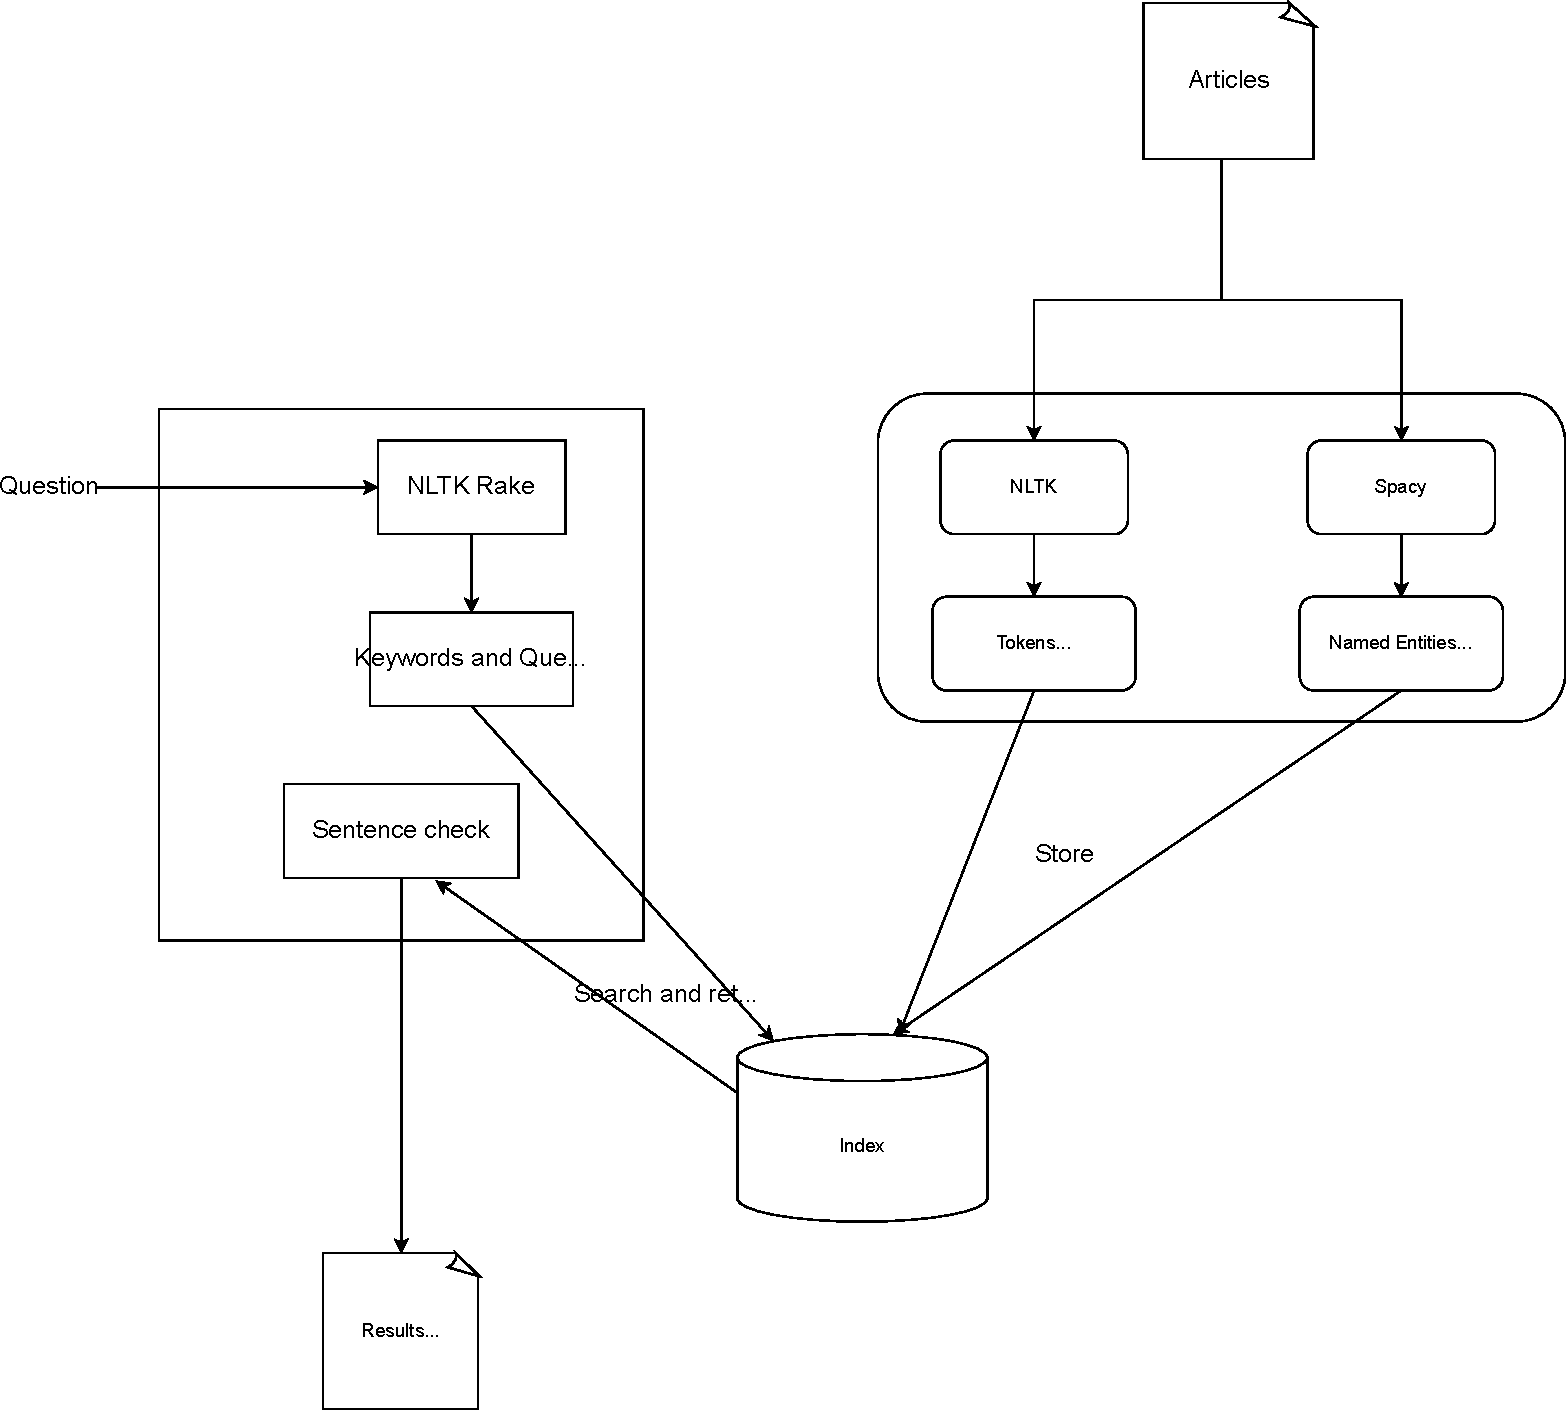
\includegraphics[width=0.9\textwidth]{fig/query.pdf}
    \caption{Architecture of Query Side Answerer}
    \label{fig:query}
  \end{figure}

  \begin{figure}[H]
    \centering
    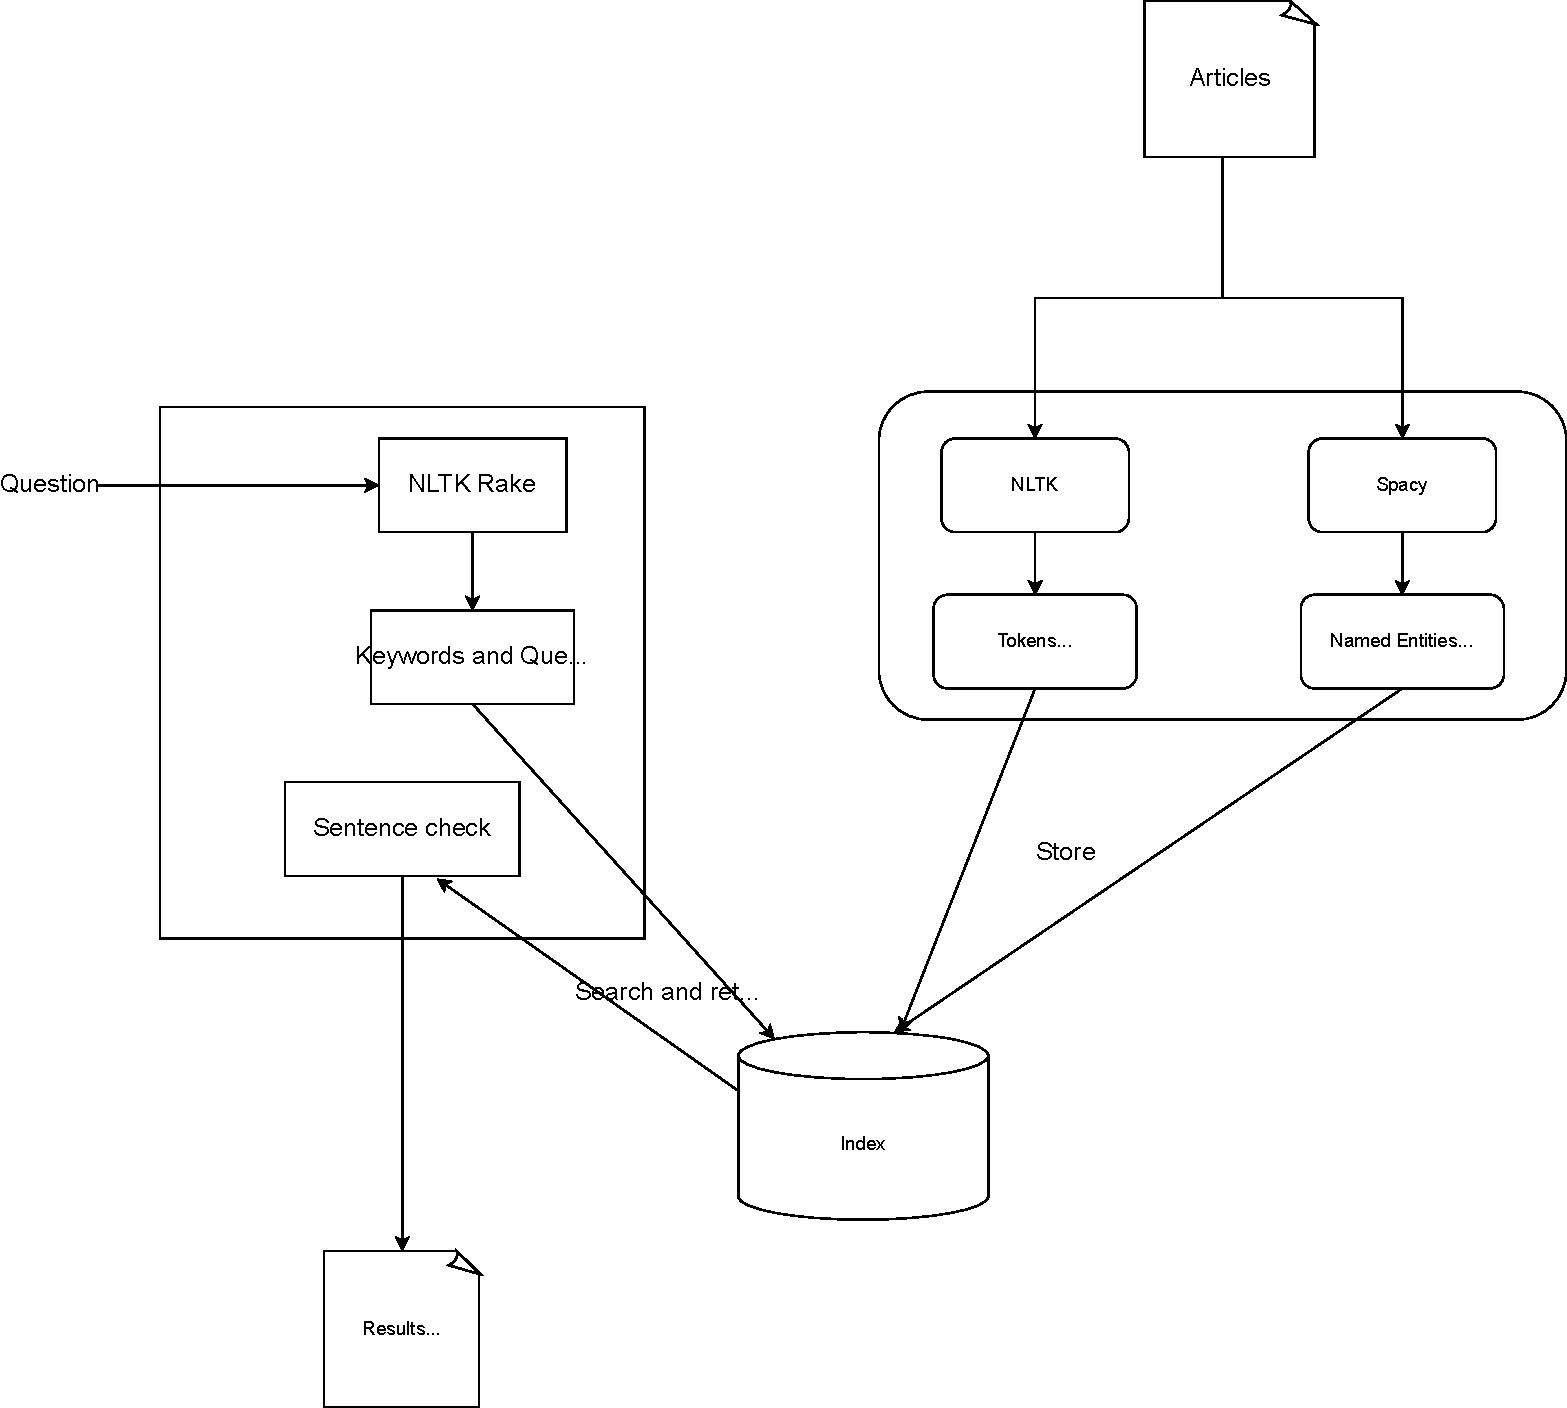
\includegraphics[width=0.9\textwidth]{fig/python.pdf}
    \caption{Architecture of Python Side Answerer}
    \label{fig:python}
  \end{figure}


\subsection{Results and Error Analysis}

An early step in development was to establish when correct articles are found. Our analysis simply counts instances of the (human-tagged) correct answer in the target sentence. This presents a small complication.

The first system we built was meant to deliberately get things wrong, and simply returned the first result in the whole \texttt{solr} database, when searching for type:'sentence'. By default, this happened to be the first sentence in article 109, ``Bird migration is the regular seasonal movement, often north and south along a flyway, between breeding and wintering grounds.'' Interestingly, because the terms ``north'' and ``south'' are answers to two unrelated questions, this method counted those as correct. Another question asked something similar, ``What is the most common direction of migration in autumn?''; the provided answer ``south'' appears in the provided answer. So we see it is an imperfect method.

Nevertheless, we used it. We tried to make data-driven decisions. As such, when we found the reasonably good, albeit very simple RAKE answerer, we began building tools for analysis. One such analysis looks at the \texttt{solr} score for a given result, and compares it when the answer is correct or incorrect, and when the article is determined correctly or incorrectly. We examined both the top score in those cases, and the deltas between scores. We did this analysis both on a small subset of questions (used for development) and the full set provided.

  \begin{figure}[H]
    \centering
    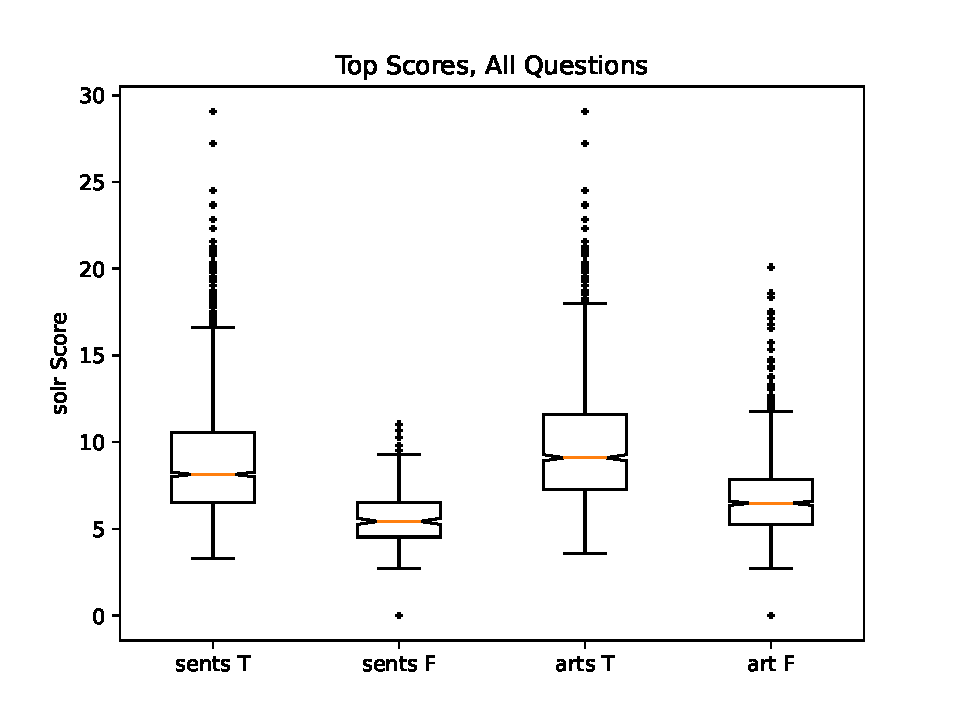
\includegraphics[width=0.8\textwidth]{fig/bt-all.pdf}
    \caption{Boxplot of Results using RAKE Answerer, Top Scores}
    \label{fig:bt-rake}
  \end{figure}

  \begin{figure}[H]
    \centering
    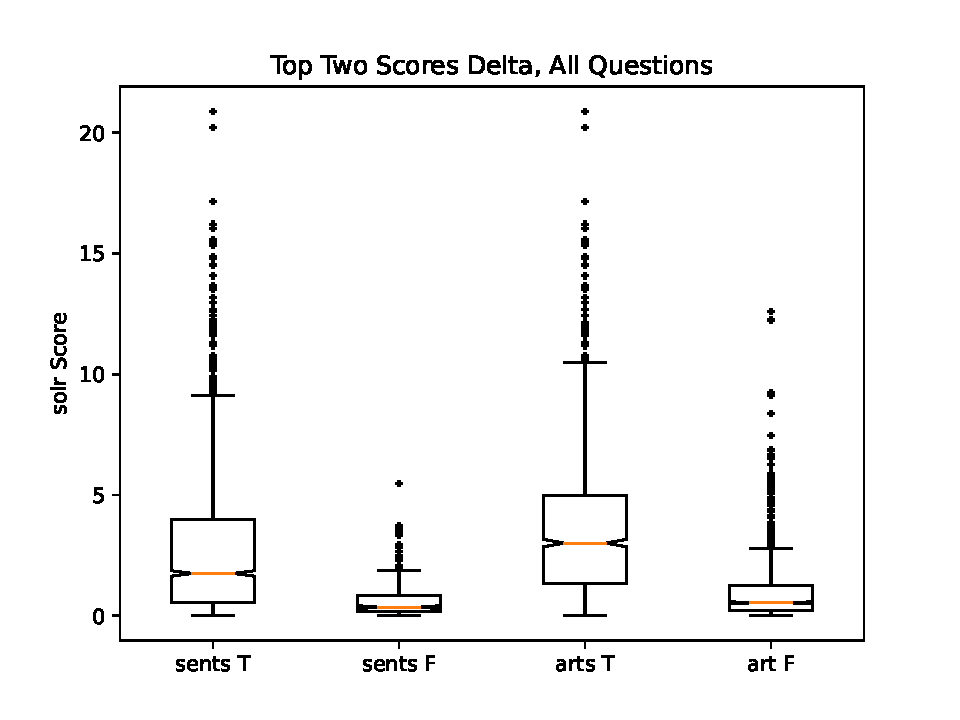
\includegraphics[width=0.8\textwidth]{fig/bd-all.pdf}
    \caption{Boxplot of Results using RAKE Answerer, Delta of Top Two Scores}
    \label{fig:bd-rake}
  \end{figure}

We examine also the Query Side answerer, and see that clearly it has worse results.

  \begin{figure}[H]
    \centering
    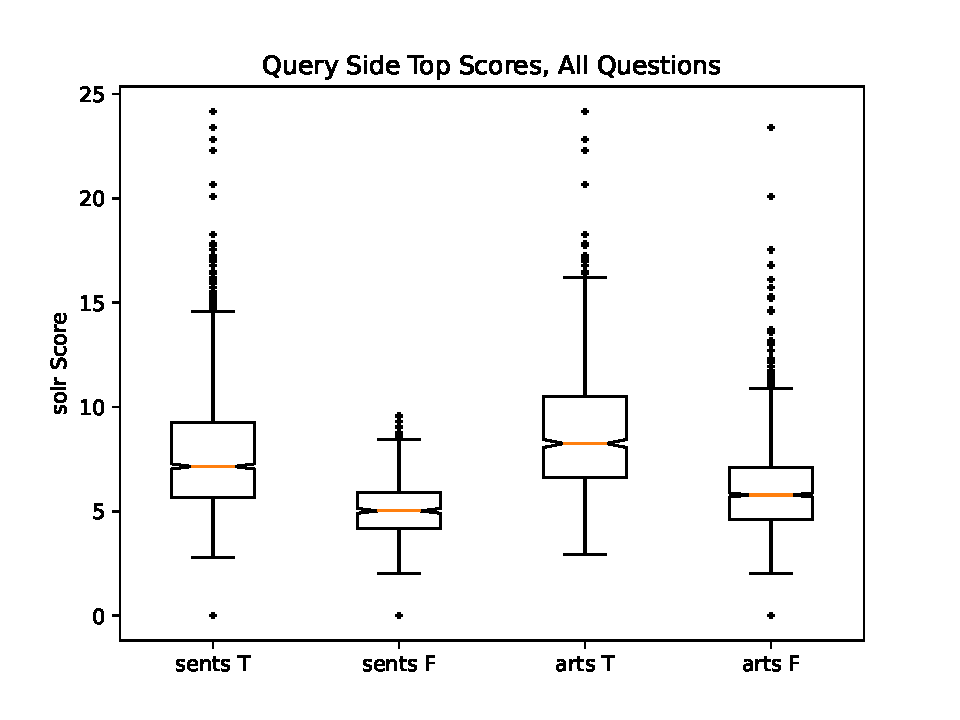
\includegraphics[width=0.8\textwidth]{fig/bt-all_query.pdf}
    \caption{Boxplot of Results using Query Side Answerer, Top Scores}
    \label{fig:bt-rake}
  \end{figure}

  \begin{figure}[H]
    \centering
    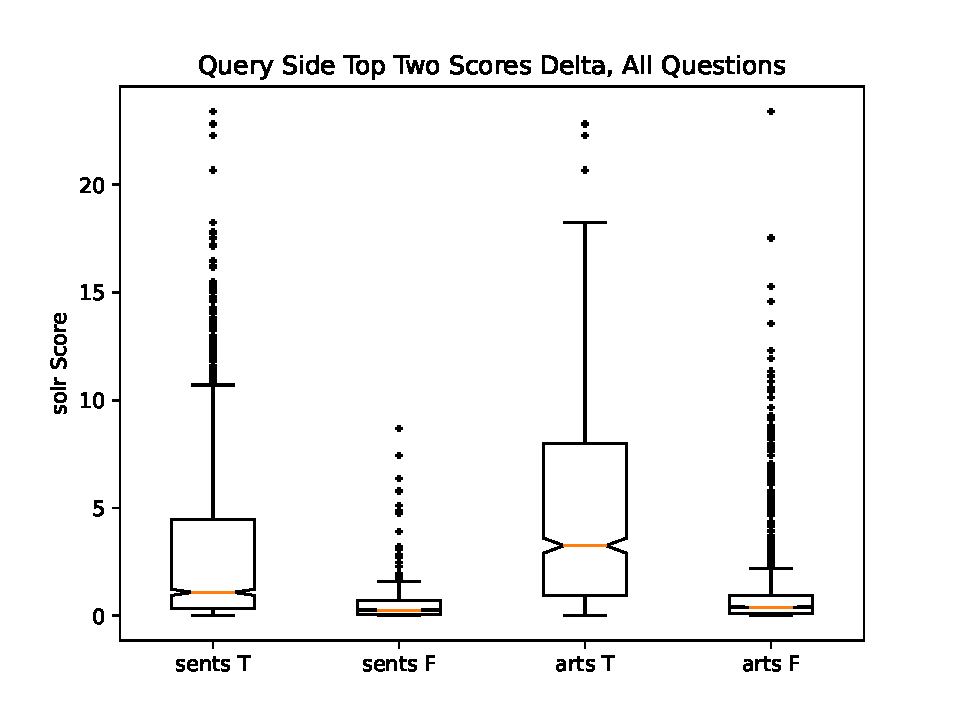
\includegraphics[width=0.8\textwidth]{fig/bd-all_query.pdf}
    \caption{Boxplot of Results using Query Side Answerer, Delta of Top Two Scores}
    \label{fig:bd-rake}
  \end{figure}


\subsection{Problems: Encountered and Resolved}

Initially, Jim had difficulty reading the data files into python, though Ziyad did not. The solution is always setting encoding='utf-8' when reading and writing files.

We built a BadAnswerer in hopes of getting the most improved award. This method simply returned the first sentence found in any article.  In the set of questions, 89 are for this article, so those are correct by default.

The initial, naive method simply using RAKE keyword search simply queried the keywords as provided. Of 2505 total questions, the correct article was found 1453 times and the correct sentence was found 769 times.

The next method broke RAKE keywords into component pieces. For instance, from the question: "On what did Skousen analyze ink and pencil remnants?" we previously found only 2 compound keywords ("skousen analyze ink" "pencil remnants"); broken up, we found 5 ("skousen" "analyze" "ink" "pencil" "remnants"). Of 2505 total questions, the correct article was found 2206 times and the correct sentence was found 1380 times. (55\%).

For the next method, we found that RAKE was identifying typical ``question words.'' Blacklisting just the two most common words ("one", "type") did not improve results.

We attempted to build in named entity utilization. Initial exploration led us to realize that the named entities identified for a sentence were often unrelated to the desired answer. For instance, the sentence containing the answer to ``Who seized the US Embassy in Iran in 1979?'' had the following named entities: 'November 4, 1979\_DATE', 'the United States Embassy\_GPE', '52\_CARDINAL', 'the United States\_GPE', 'Mohammad Reza Pahlavi\_PERSON', 'Iran\_GPE'. Note that the correct answer, ``students'' were not named. More examples are available in the appendix.


There is a list of questions, below, with multiple question words in a single question. Need to use better system (POS tagging? syntatic analysis?)

Some difficulty when trying to find meronyms and holonyms... because it's not quite as simple as that. More hours than I'm proud to admit were spent debugging, when in fact the proper solution is that wordNet breaks meronyms and holonyms into substance and part types.

Adding named entities to the search didn't seem to improve things. On investigation, it was clear that the named entity types we sought we not actually set as named entities in the sentences. Perhaps this is a failing of the way we implemented named entitty detection.

\subsection{Pending Issues}

We tried to apply scipy statistics to the score results, but get ridiculous and plainly incorrect p-values and confidence intervals (overestimating precision).

We were unable to finish integrating the python and query side approaches.

\subsection{Potential Improvements}

Currently, the overlap metric produces results with the same values. These need to be differentiated.

The method by which the statistics were generated could be significantly improved, which would give better error tolerances for the extant query-side method. This would involved running through the tiers iteratively and producing data.

In the tier iteration method, we intended to, but were unable to implement a final tier using synonyms of verbs.

The rake blacklist could be expanded greatly.

Further work would employ more of the techniques found in \texttt{Falcon}, 2000 \cite{falcon2000}.

\HomeworkHeader{Appendix}{}

The following are examples of insufficient named entities.

\begin{lstlisting}
Naive checking of named entities in the answer gives poor results. the following questions have the correct answer in the top result, but the associated NE would remove them from consideration:
'Of what was Magadha one of sixteen?'
['one\_CARDINAL', 'sixteen\_CARDINAL', 'India\_GPE']

'Who seized the US Embassy in Iran in 1979?'
['November 4, 1979\_DATE', 'the United States Embassy\_GPE', '52\_CARDINAL', 'the United States\_GPE', 'Mohammad Reza Pahlavi\_PERSON', 'Iran\_GPE']

'What type of government did Espartero have?'
['Maria Cristina\_PERSON', 'Espartero\_PERSON', 'Spain\_GPE', 'two years\_DATE', '18th\_ORDINAL', '16 September 1840 to\_DATE', 'May 1841\_DATE']

'On what did Skousen analyze ink and pencil remnants?'
['the Community of Christ-RLDS Church\_ORG', 'Independence\_GPE', 'Missouri\_GPE']

'Who ordered Valencia punished for supporting Charles?'
['25 April 1707\_DATE', 'English\_NORP', 'Valencia\_PERSON', 'Philip\_PERSON', 'Valencia\_PERSON', 'Charles of\_PERSON', 'Austria\_GPE']

'What is the natural gas condensate used to dilute bitumen?'
(no named entities)

'When did the Ming hold the divide and rule policy?'
['Luciano Petech\_PERSON', 'Sato Hisashi\_PERSON', 'Tibet\_GPE', 'Sakya\_ORG']

'What does an inker do?'
['American\_NORP']

'What was a normal play time per side for LPs?'
['up to 30 minutes\_TIME', 'about 22 minutes\_TIME', 'about forty-five minutes\_CARDINAL']
\end{lstlisting}

\bibliography{my}{}
\bibliographystyle{plain}

\end{document}